\documentclass{article}


\usepackage{/Users/RobThomas/Documents/Latex/bathdronereport}
%% Helvetica
\usepackage[scaled]{helvet}
\renewcommand\familydefault{\sfdefault} 
\usepackage[T1]{fontenc}
\usepackage{listings}
\usepackage{caption}
\usepackage{wrapfig}
\usepackage{subcaption}
\usepackage{graphicx}
\usepackage{subfiles}


%% Change colour of sections
\usepackage{sectsty}
%% Set colours
\sectionfont{\color{BathBlue}}
\subsectionfont{\color{BathBlue}}
\subsubsectionfont{\color{BathBlue}}

\lstset{
	basicstyle=\scriptsize,
    frame=single,
    breaklines=true,
    numbers=left,
    numbersep=8pt,
    numberstyle=\tiny,
    postbreak=\raisebox{0ex}[0ex][0ex]{\ensuremath{\color{red}\hookrightarrow\space}}
}

\degree{Candidate Number : 10374}
\module{EE40054 - Digital Image Processing}
\title{Noise Reduction of Synthetic Aperture Radar (SAR) and Ultrasound Images}
\subtitle{Technical Report}

\begin{document}



\maketitleBTH

\section{Introduction}
The human vision system is both very sophisticated and highly complicated yet it is not perfect. Noise, the bane of many digital systems but especially image processing, can obfuscate images making them difficult to process by eye when gradients and edges are blurred. Noise, however, typically follows pseudo-random distributions and as such can be counteracted through the use of certain filters. Even in the absence of noise, filters have many uses for enhancing images by artificially exacerbating the gradients and edges that the human vision system has evolved to detect.  


\section{Sample Images}
In the initial assignment brief the two images NZjers.png and foetus.png\cite{Evans:aa}. For further appraisal DropZone.png was selected (taken from footage of an inflight aUAS \cite{Thomas:aa}) and in order to assess the potential reactions to noise 20\% gaussian noise was applied to foetus.png. All of these images are displayed in figure \ref{fig:newPic}.


\begin{figure}[h]
\begin{subfigure}{.5\textwidth}
	\centering
	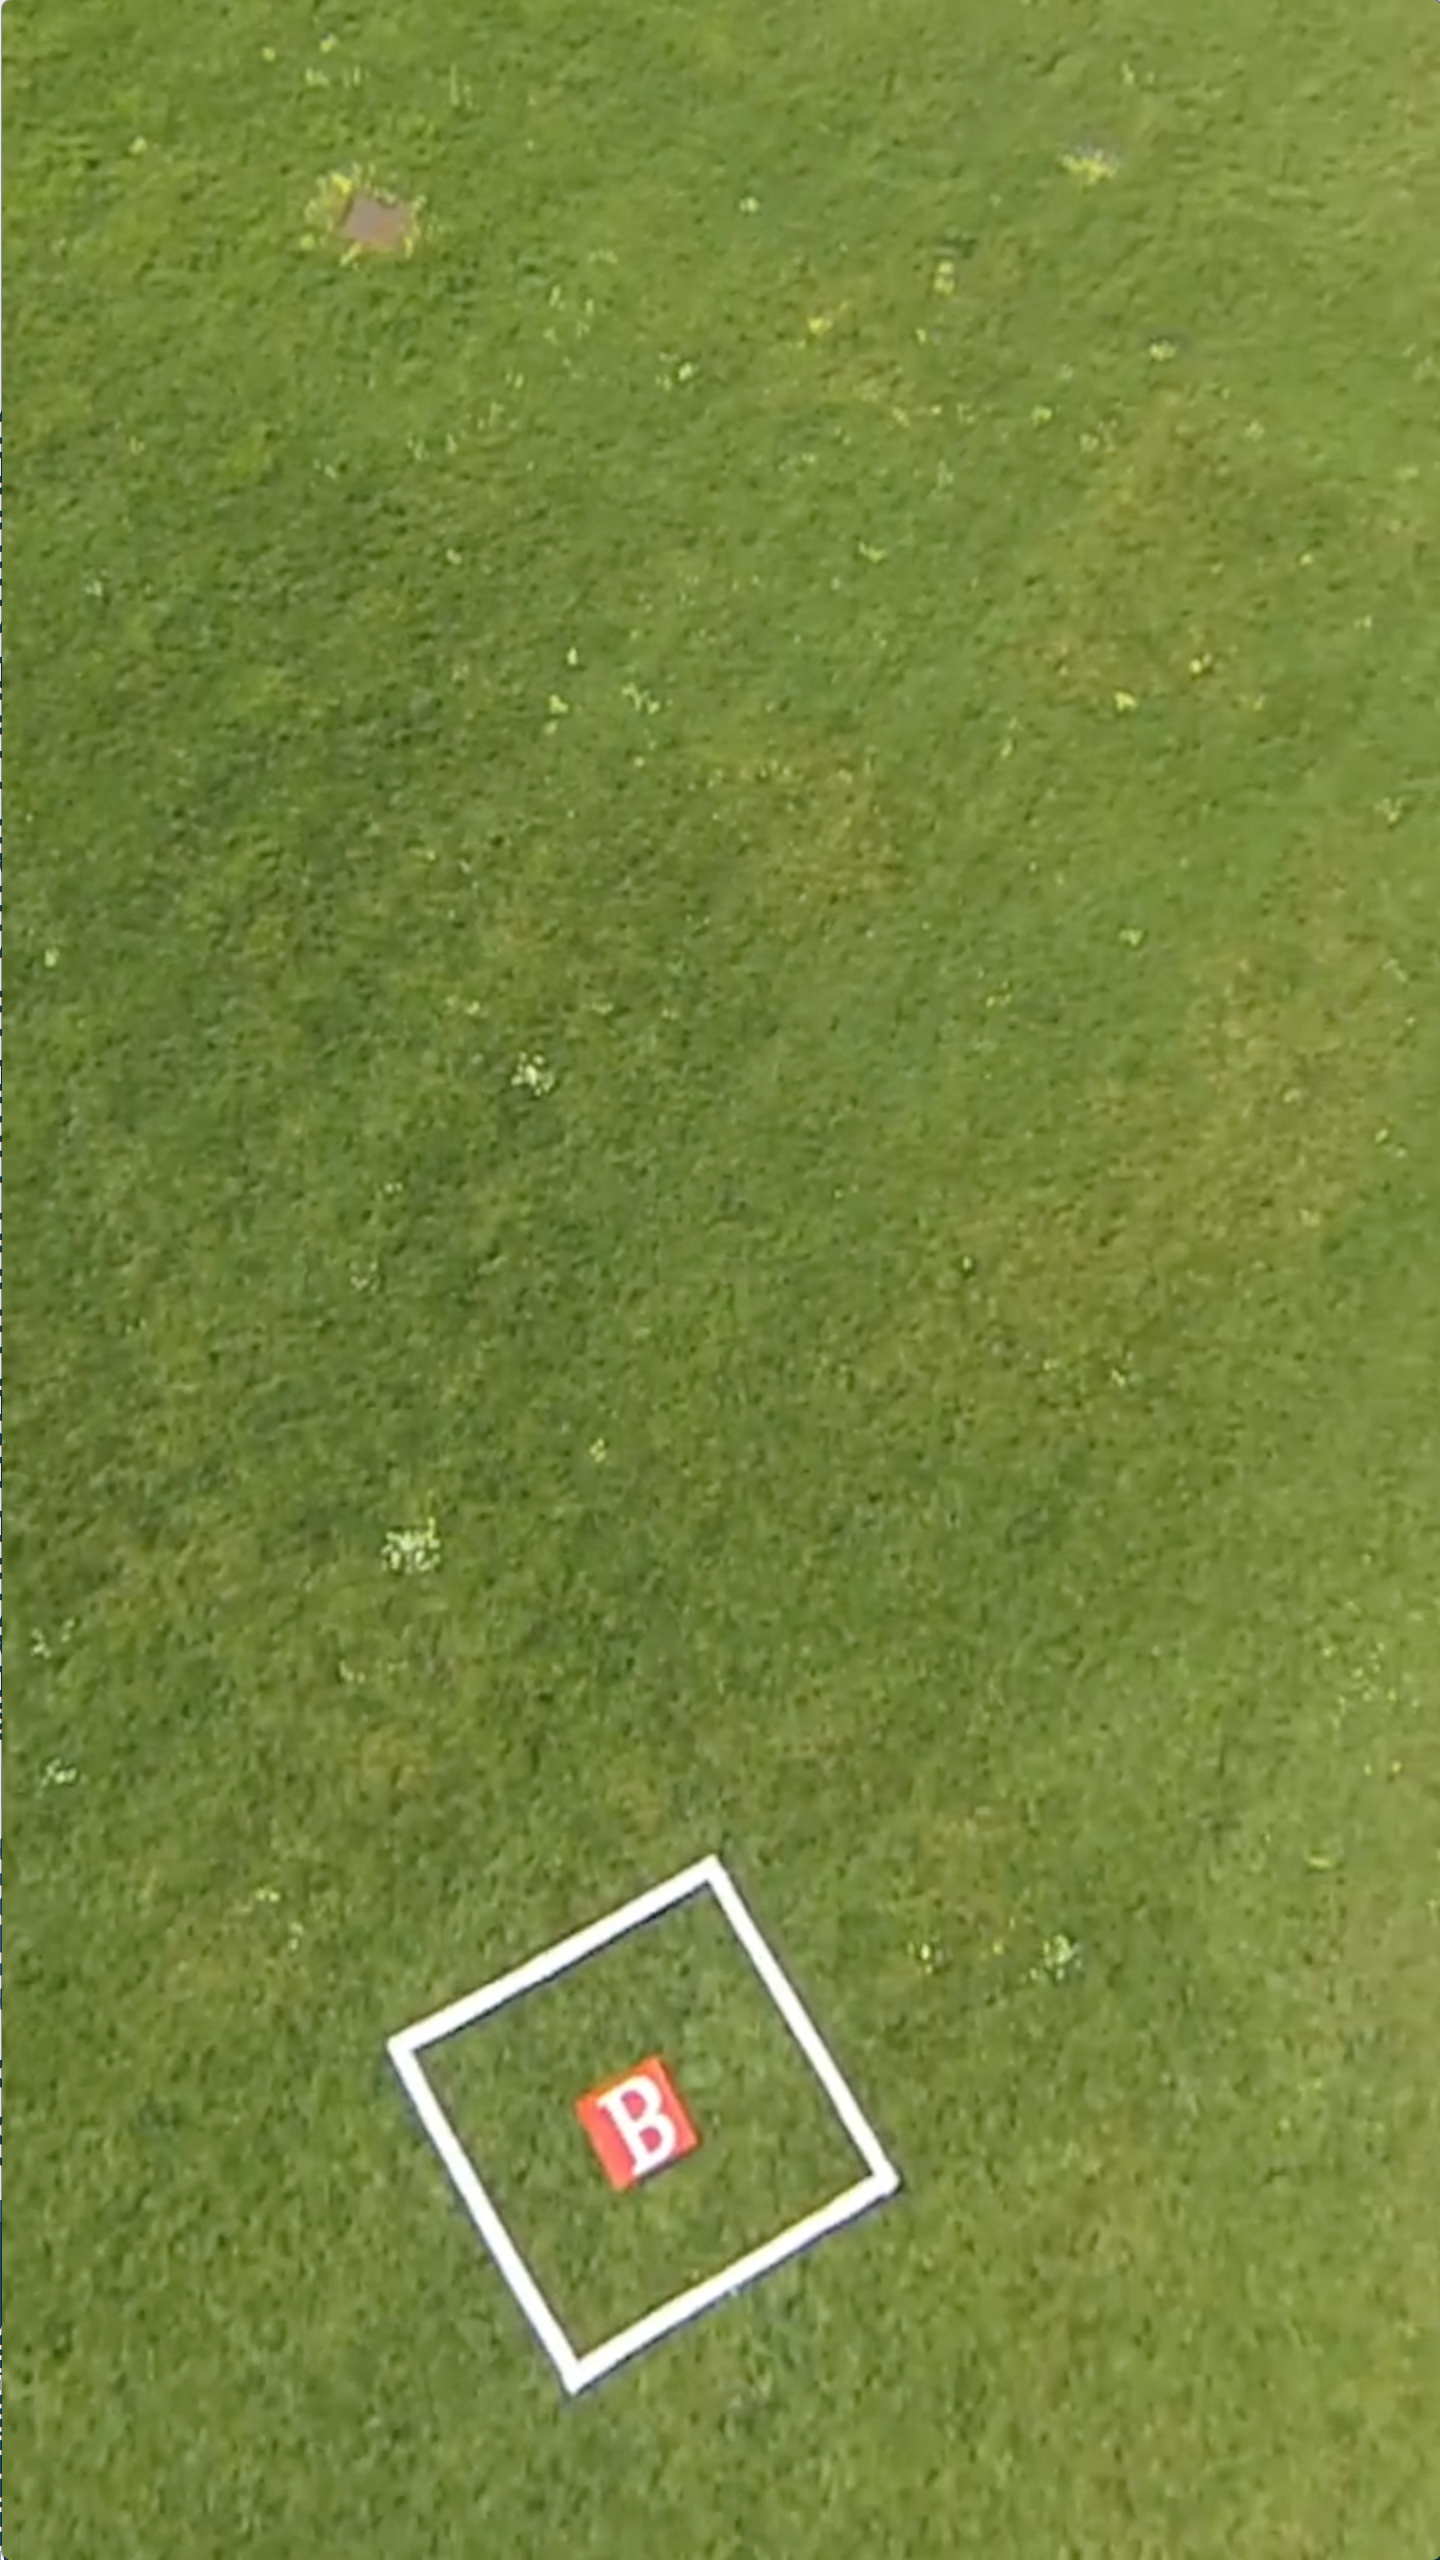
\includegraphics[width=.8\linewidth]{BaseImages/DropZone.png}
	\caption{Sample image from Team Bath Drones}	
\end{subfigure}
\hfill
\begin{subfigure}{.5\textwidth}
	\centering
	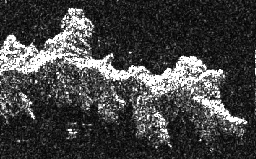
\includegraphics[width=.8\linewidth]{BaseImages/NZjers1.png}
	\caption{Provided image NZjers1.png}	
\end{subfigure}


\begin{subfigure}{.5\textwidth}
	\centering
	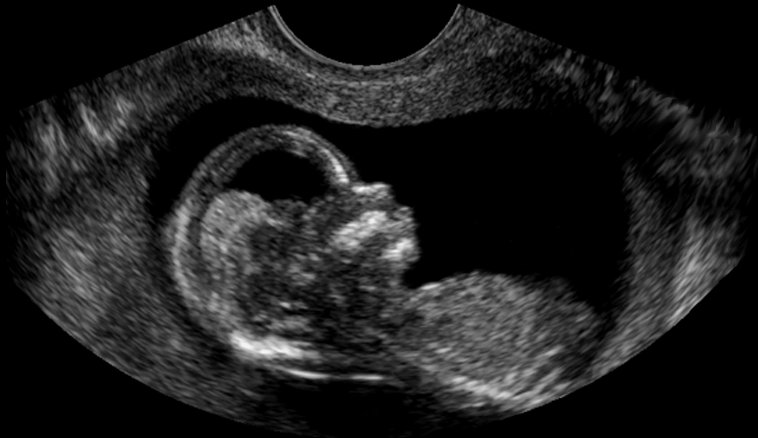
\includegraphics[width=.8\linewidth]{BaseImages/foetus.png}
	\caption{Provided image foetus.png}	
\end{subfigure}
\hfill
\begin{subfigure}{.5\textwidth}
	\centering
	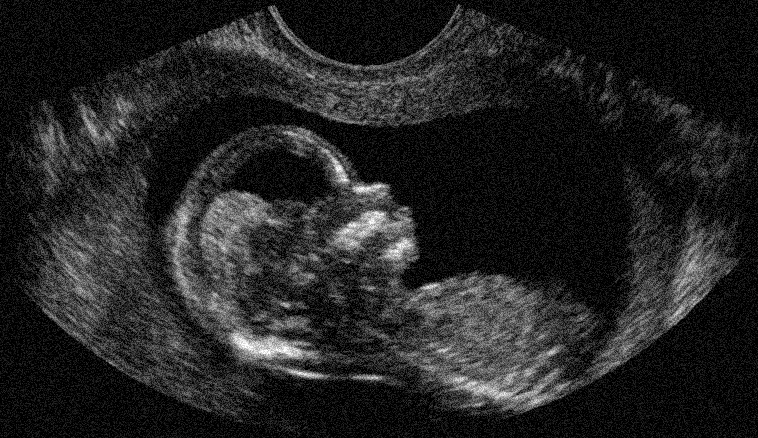
\includegraphics[width=.8\linewidth]{BaseImages/foetusNoise2.png}
	\caption{foetus.png with 20\% gaussian noise}	
\end{subfigure}

\caption{The images used for comparing filters}
\label{fig:newPic}
	
\end{figure}

\section{Filters}



\subsection{Comparison of Mean, Median and Gaussian Filters}
Comparing the mean filter, the median filter and the gaussian filter for an equivalent window size on the image foetusNoise2 we are able to see the clear differences in the 3 filters. Comparing the gaussian and the mean filters for windows of the same size the mean filter is producing a much greater amount of blurring and edge reduction than the gaussian whereas the gaussian filter has retained a large amount of the noise in the original image. To achieve the same blurring of the edges as seen in the mean filter we have to vastly increase the size of the gaussian window, when we do this we see a lot of the noise disappear from the image with regards to the edges, however inspecting the image itself we see the contrast is still superior to the mean filter. 

\begin{figure}[h!]
	\centering
	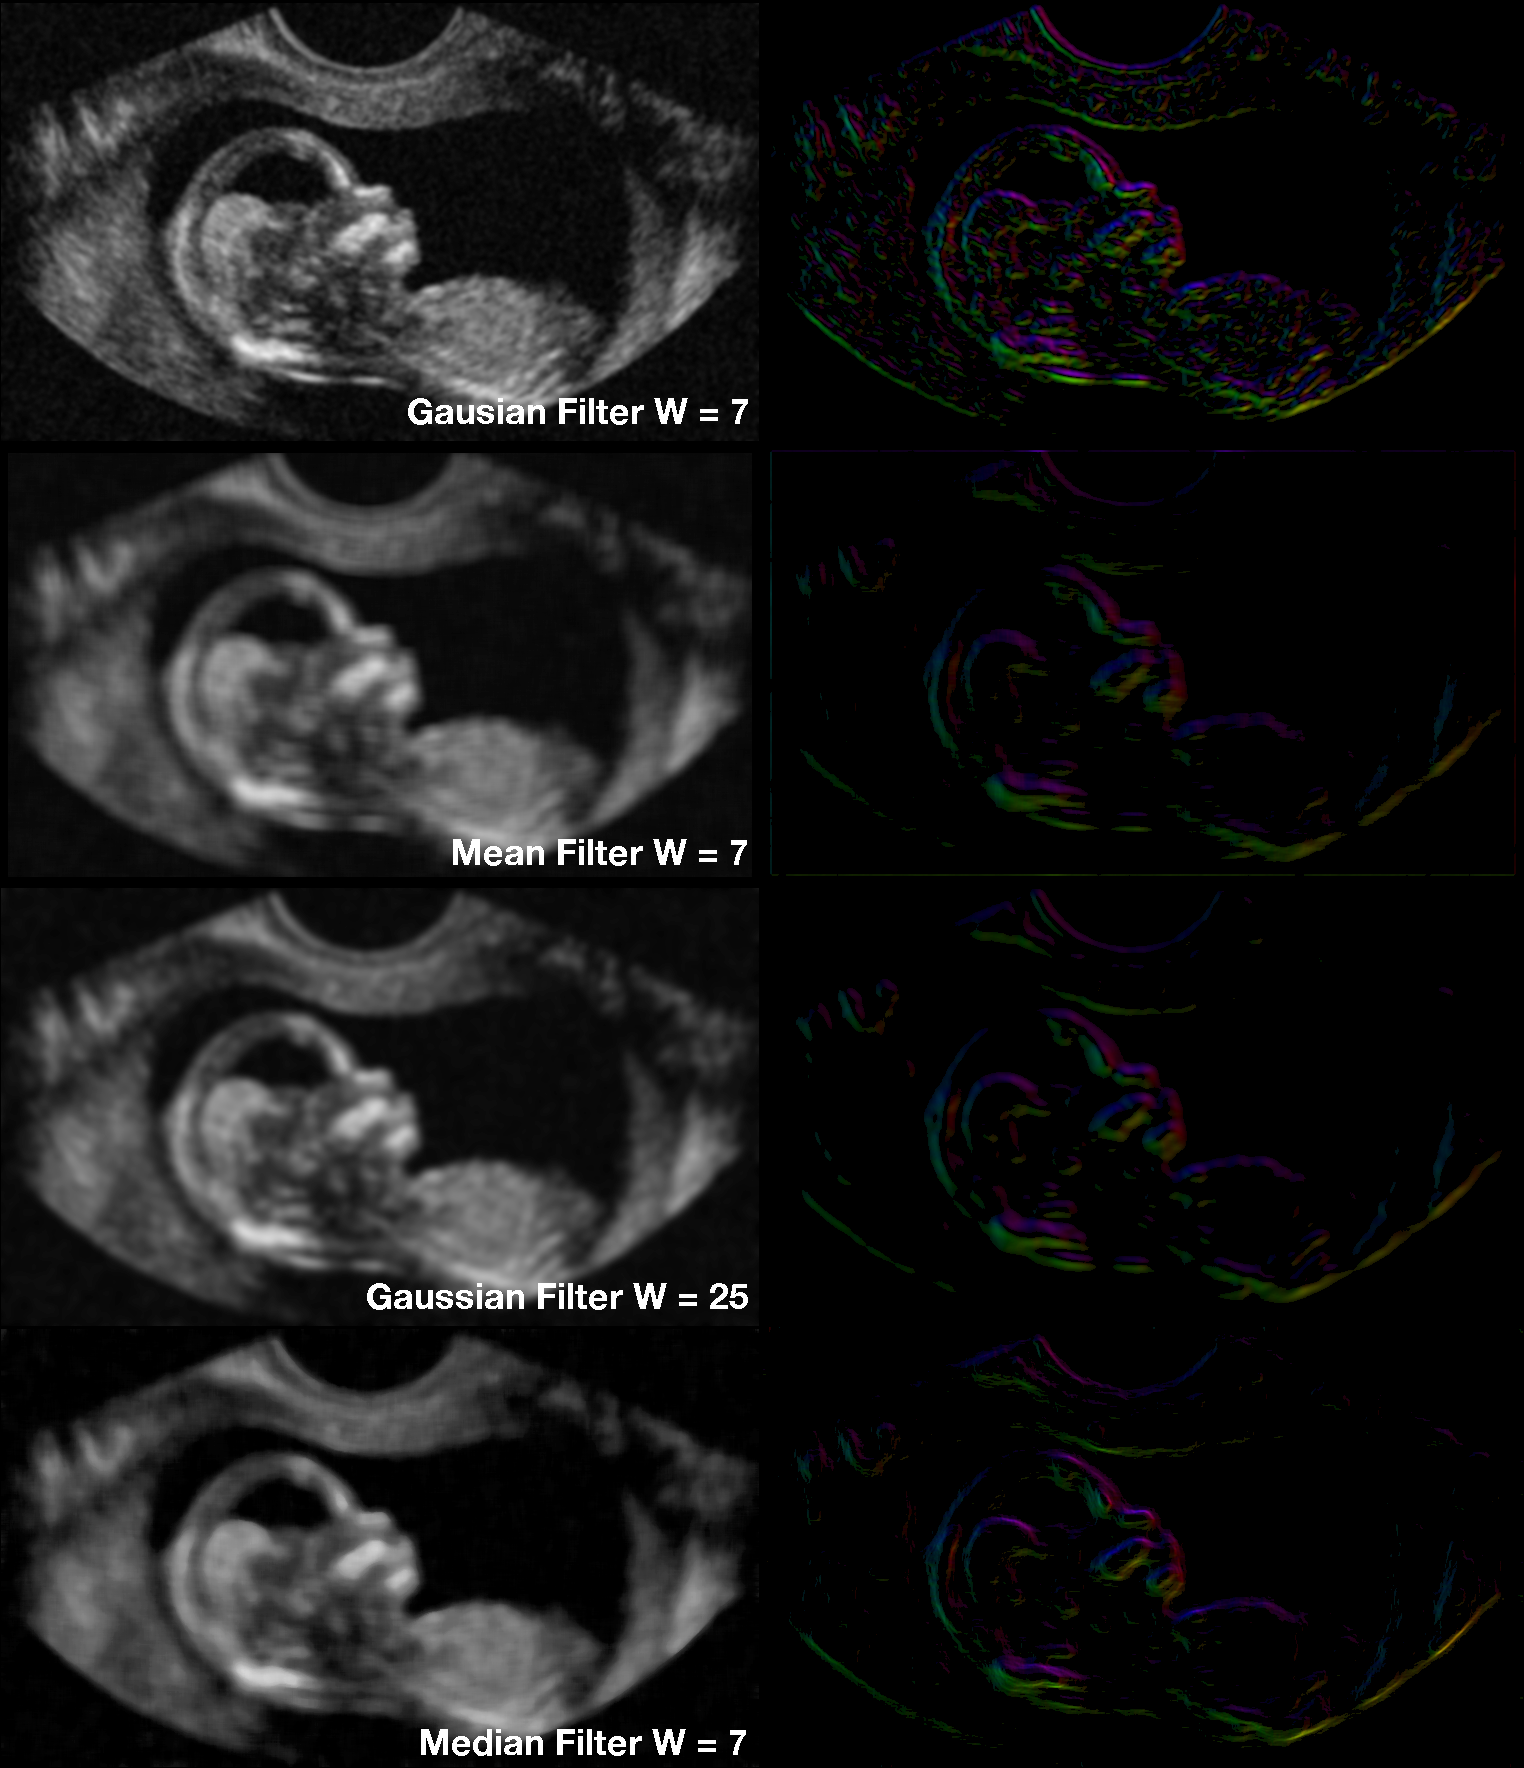
\includegraphics[width = \textwidth]{FilterCompare}
	\caption{Comparison of a range of filters, minimum gradient = 25}
	\label{fig:FilterCompare}
\end{figure}

Lastly we have the median filter for window size 7. Of all of the images presented this has the most clearly defined edges with the skull, cheekbone and the mass within the skull all well defined, we are also able to see that the line surrounding the image is much thinner, being closer to the gaussian for small window size. 



\subsection{Truncated Mean Filter}

By removing outliers within a window before calculating the mean of that window the potential for noise or nearby points of luminescence/darkness adjusting the mean is diminished. Comparing the images in figure \ref{fig:TrimmedMean} we can see how edges are better preserved in the image. Furthermore the shadows on the bottom side of the image and the lighter ridges are much more visible.

\begin{figure}[h]
	\centering
	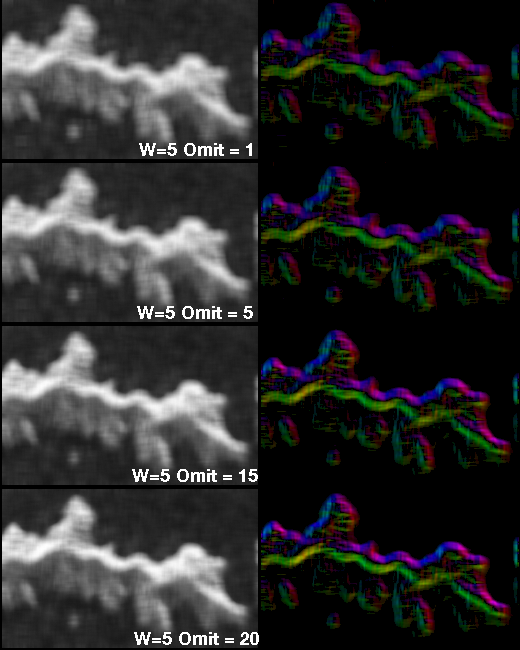
\includegraphics[width = 0.6\textwidth]{ShortMean2}
	\caption{Comparing different amount of values omitted in calculating the mean of a 11x11 image}
	\label{fig:TrimmedMean}
\end{figure}

\subsection{Adaptive Weighted Median}
\begin{figure}
\centering
$\ W_{i,j} = W_{mid} - d * c * \frac{\sigma}{\mu} $\	
\caption{Adaptive Weighting Median, Weighting function}
\label{fig:ADMedFUNC}
\end{figure}


By adjusting the weights for median values based upon the characteristics of the window it is possible to improve the noise response for the median filter on a window by weighting the values within it in accordance with the properties of that window using the equation shown in figure\ref{fig:ADMedFUNC} \cite{Gonzalez:2016aa}. Shown in figure \ref{fig:MedComp} the median and adaptive weighted median filters have both been applied to the image \textit{foetus.png} and from visual inspection of both the output images and their Sobel detected. edges it is clear to see a notable improvement to the clarity of the image.


\begin{figure}[h!]
	\centering
	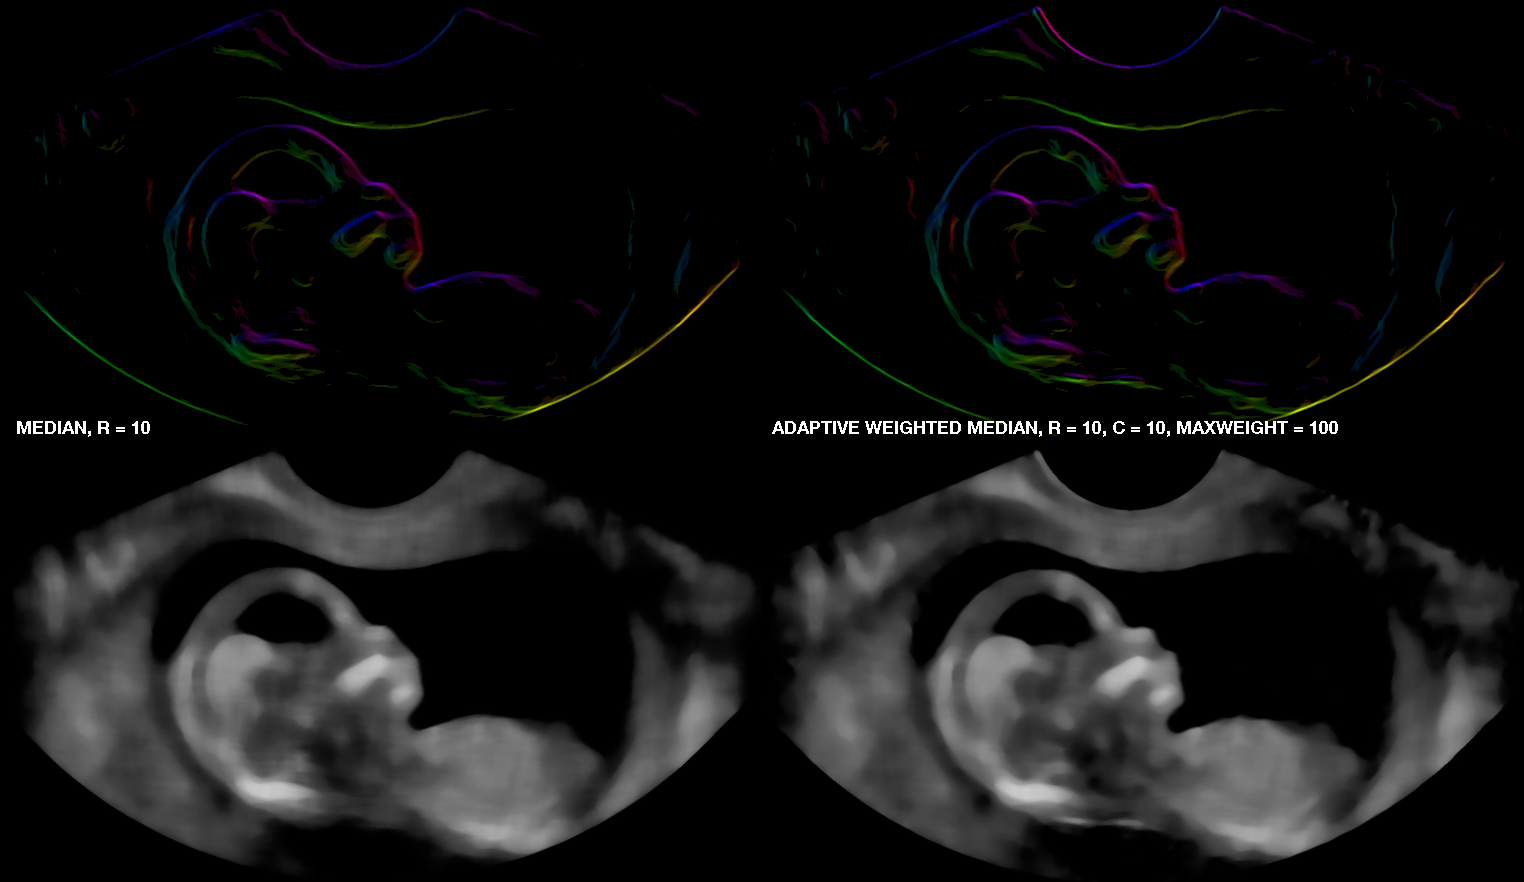
\includegraphics[width = 0.8\textwidth]{MedComp.png}
	\caption{Comparison of the Median and Adaptive weighted Median filters with the same window size on the image: foetus.png}
	\label{fig:MedComp}
\end{figure}

When these filters are re-run over the image with 20\% gaussian noise added to it we see an even greater improvement in the edges visible, the facial structure is clearly defined as and the spinal section of the foetus is notedly separated from the background in comparison to the simple mean filter

\begin{figure}[h!]
	\centering
	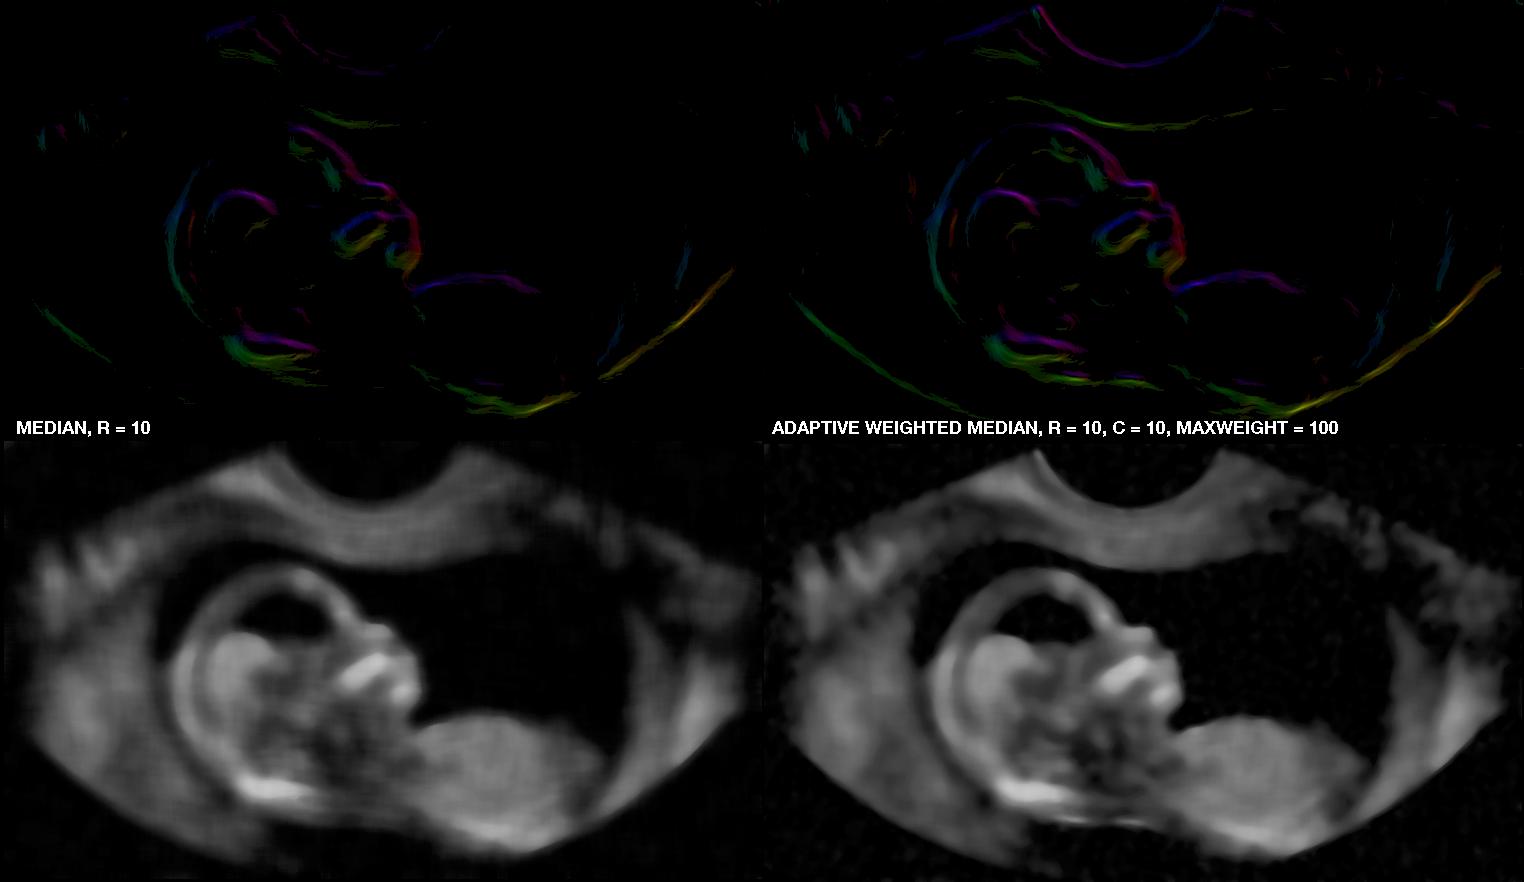
\includegraphics[width = 0.8\textwidth]{MED2COMP.png}
	\caption{Comparison of the Median and Adaptive weighted Median filters with the same window size on the image: foetus.png with 20\% Gaussian Noise}
	\label{fig:MED2COMP}
\end{figure}




\section{Edge Detection}


\begin{figure}[h]
\begin{subfigure}{.5\textwidth}
	\centering
	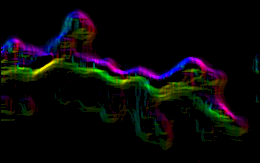
\includegraphics[width=.8\linewidth]{PreComp.png}
	\caption{Prewitt Filter}	
\end{subfigure}
\hfill
\begin{subfigure}{.5\textwidth}
	\centering
	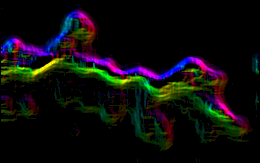
\includegraphics[width=.8\linewidth]{SobComp.png}
	\caption{Sobel Filter}	
\end{subfigure}
\caption{Comparison of Sobel and Prewitt edge filters applied to the image \textit{NZjers.png} after a median filter (w=7)}
\label{fig:EdgeCompare}
\end{figure}

In order to more easily assess the information retained within the image after filtering edge detection methods were coded into the image class. Comparing the Sobel and Prewitt methods gave very little detectable difference with regards to the outputted image however due to the edges appearing to have greater visibility, figure \ref{fig:EdgeCompare}, the Sobel filter was selected. In order to better visualise the gradients the theta angle generated by the method was encoded as the hue value in an HSV image, with the gradient value itself being assigned as the Value. Saturation was set to 255 across the image to aid in readability. Figure \ref{fig:SobDrop} below shows the edge filter applied to the DropZone image after a median filter (w=7) was applied, not only are the outlines of the white square in the image clearly visible but the lines themselves clearly show the direction of their gradients. Unfortunately the initial conversion to grayscale makes the red square very difficult to distinguish from the grassy backdrop.
\begin{figure}[h!]
	\centering
	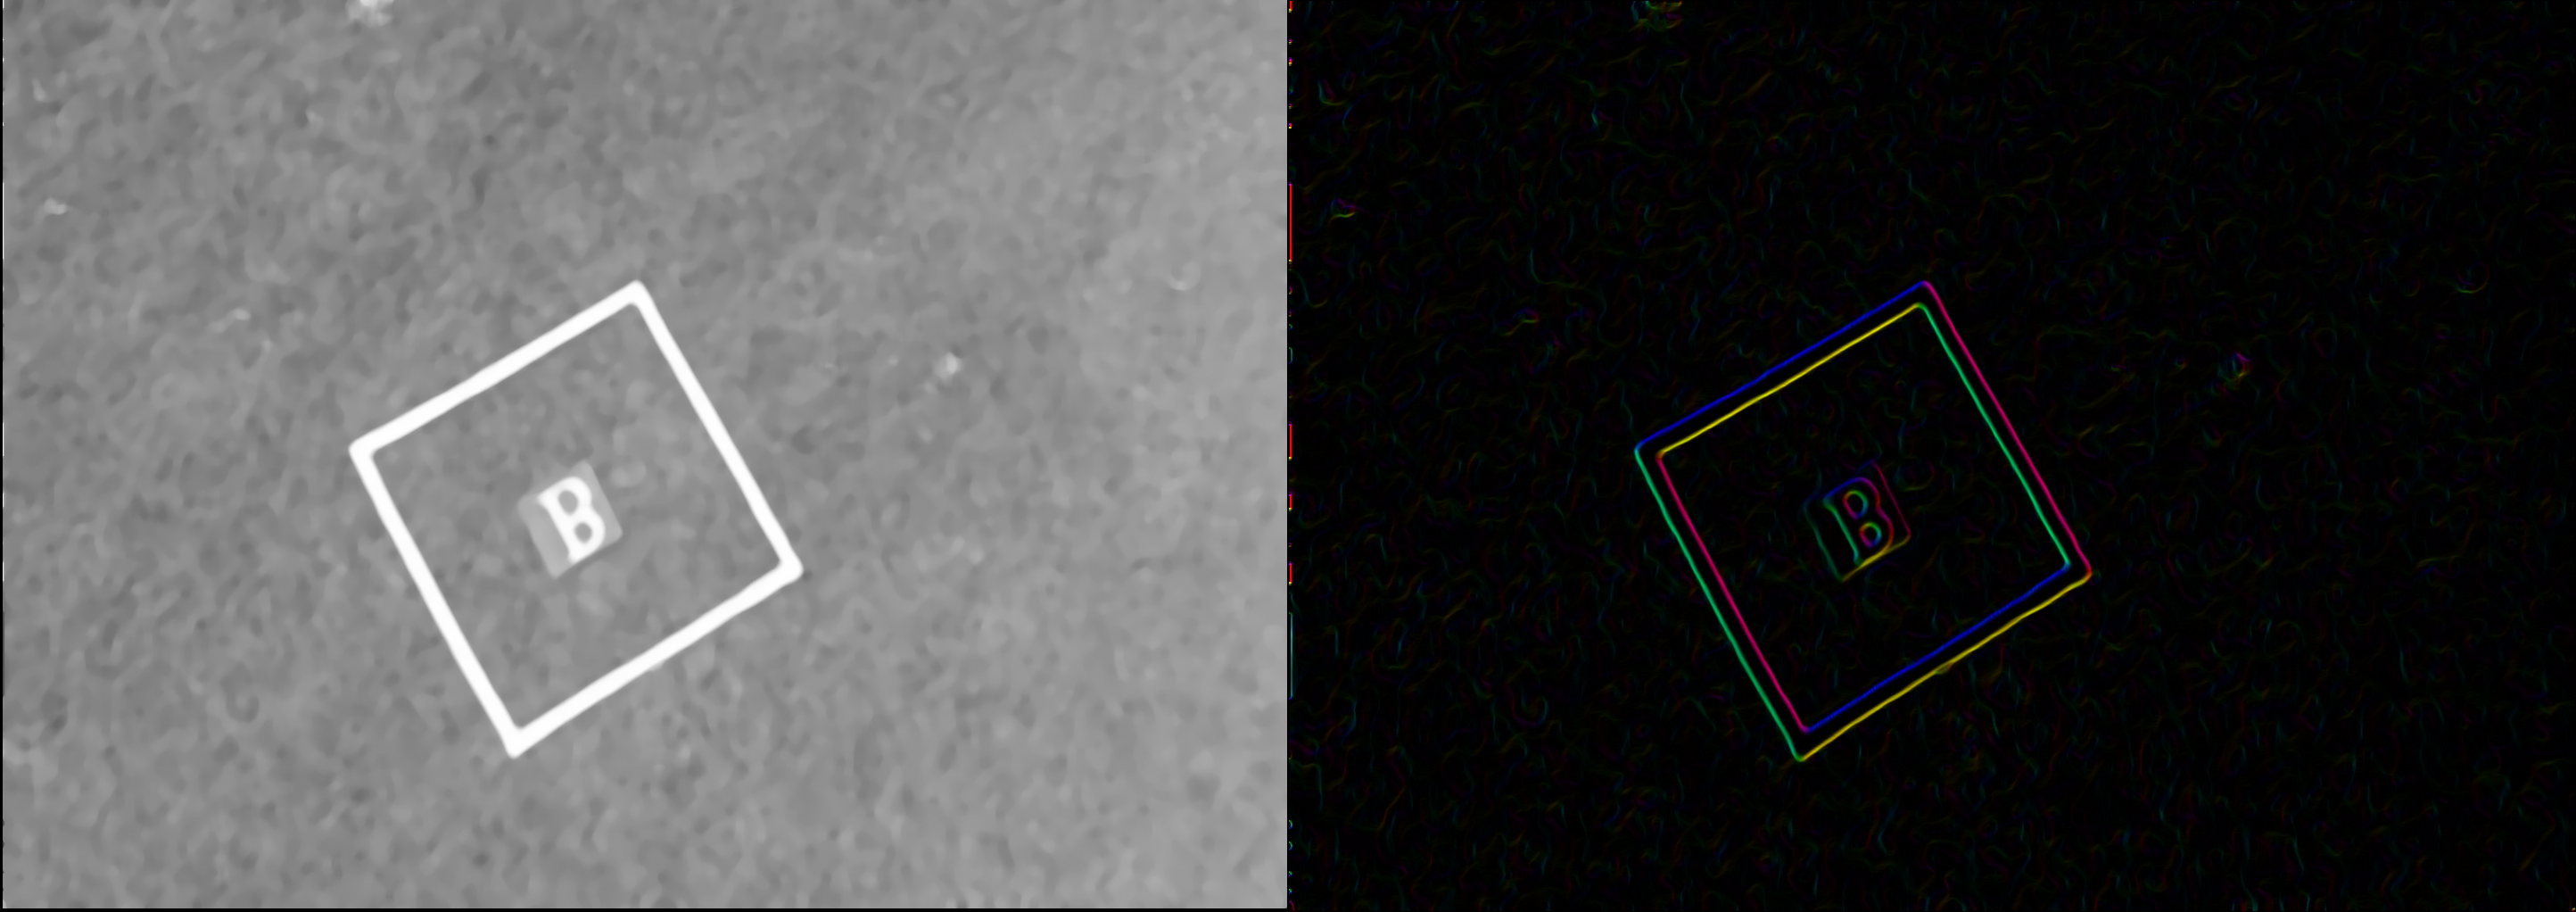
\includegraphics[width = \textwidth]{SobelDropComp}
	\caption{Example of the Sobel edge detector applied after a median filter (w = 7) on the image DropZone.png}
	\label{fig:SobDrop}
\end{figure}

With more noisy images it is important to apply a degree of thresholding to the gradients required to count as an edge. Shown in figure \ref{fig:ThreshComp} it can be seen that only a low threshold is needed to remove the lower values of noise however

\begin{figure}[h]
	\centering
	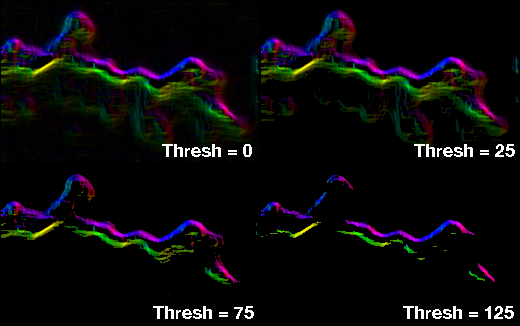
\includegraphics[width = 0.8\textwidth]{ThreshComp}
	\caption{Comparing the effects of minimum gradient thresholds on the Sobel edge detector}
	\label{fig:ThreshComp}
\end{figure}


\newpage
\section{Evaluation}

From the analysis of the different filters it was determined that the adaptive weighted median gave the most consistently good results for improving the images. For both the initially provided images there is a very clear improvement in the edge detection and readability of the images.


\begin{figure}[h!]
	\centering
	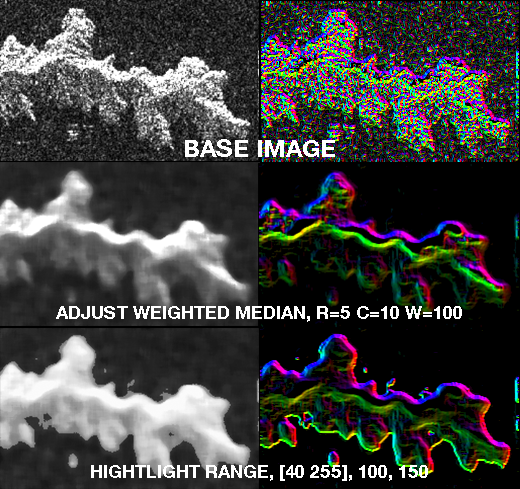
\includegraphics[width = 0.6\textwidth]{SUPERNJ.png}
	\caption{Comparing Stages of image analysis on \textit{NJzers1.png}}
	\label{fig:SuperNJ}
\end{figure}

However if, in both cases, we determine that we care most about the edges between the objects in the image and the background then the application of a range highlight filter can help aid separating the objects from the backgrounds. The results of these range highlights can be seen in figure \ref{fig:SuperNJ} and figure \ref{fig:MegaFOET}. 

\begin{figure}[h!]
	\centering
	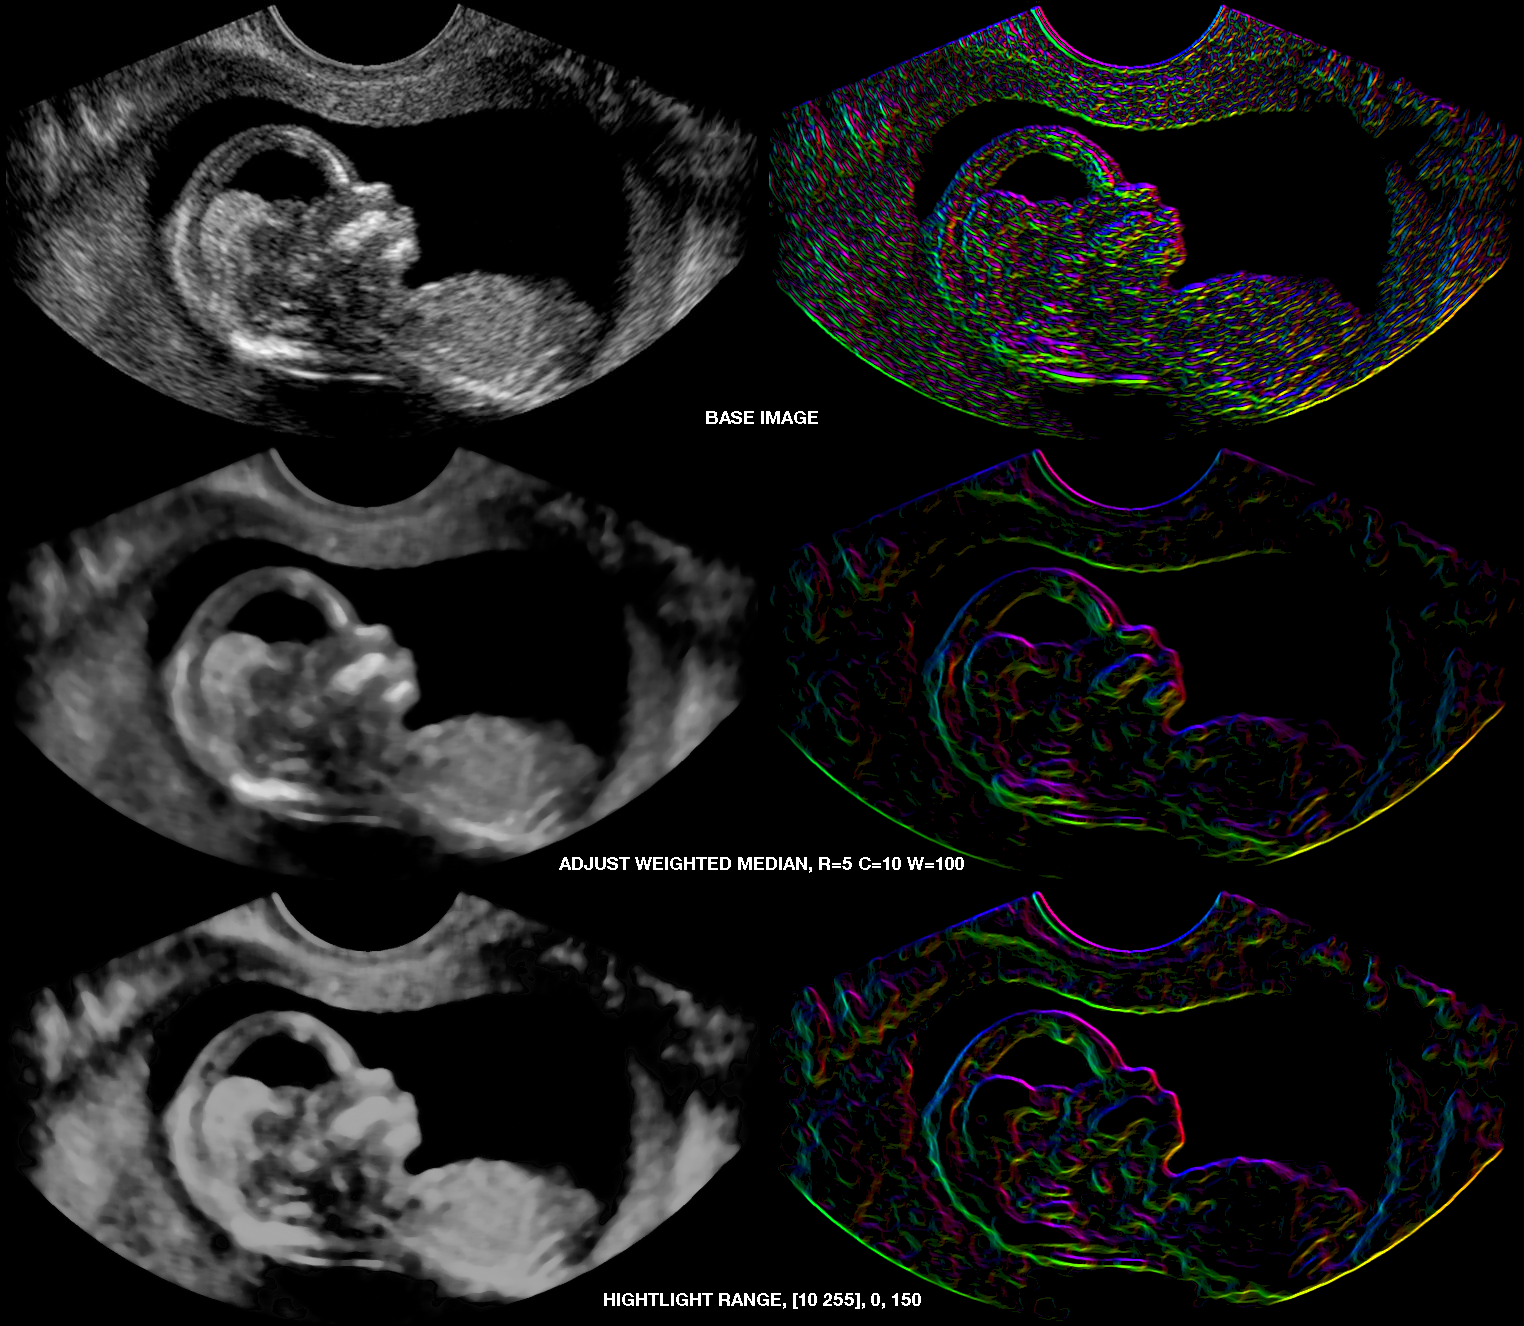
\includegraphics[width = 0.8\textwidth]{MEGAFOET.png}
	\caption{Comparing Stages of image analysis on \textit{foetus.png}}
	\label{fig:MegaFOET}
\end{figure}




\section{Image Class}
The image class is used to apply filters onto an imported image and to log all of the transforms performed. The methods are detailed in the subsections below. 

\subsection{Universal Functions}
These functions were either used for the initialisation of the image class or for common minor adjustments to the image.
\begin{enumerate}
	\item{\textbf{\_listFiles(\*args)}} This function lists all png files within the current working directory to aid in loading image files.
	\item{\textbf{\_importPic(\*args)}} Using OpenCV's imread function this imports a grayscale copy of the image specified.
	\item{\textbf{\_printFileList(\_,listOfFiles)}} Prints the list of all images found within the current directory.
	\item{\textbf{\_genborders(self,amount)}} Function to create a border around the image by mirroring the contents out for a distance of \textit{amount} pixels.
	\item{\textbf{\_deborders(self,amount)}} Function to remove a border for a distance of \textit{amount} pixels.
	\item{\textbf{createWindows(self, windowSize)}} Function that creates an array of all windows within an image of size $\ 2*windowSize +1 $\ .
\end{enumerate}

\subsection{External Functions}
These functions were used for large scale manipulations of the images such as applying masks, updating the image or getting the dimensions of the image.
\begin{enumerate}
	\item{\textbf{imageSize(self)}} Returns the dimensions of the grayscale image.
	\item{\textbf{uodateImage(self, newImage, transform)}} Updates the image in the structure with a new image and appends the transform provided to the list of all applied transforms.
	\item{\textbf{duplicate(self)}} Returns a new image with the same image as the original image. 
	\item{\textbf{mask(self, mask)}} Applies a mask provided to the image
	\item{\textbf{overlay(self,imageOver,mask)}} Overlays imageOver ontop of the current image in the structure in accordance to the mask provided.
	\item{\textbf{snrRatio(self)}} Small function that prints and returns the current signal to noise ratio of the image.
\end{enumerate}

\subsubsection{Output Functions}
These functions were used to display the outputs of the processed images or save to files.
\begin{enumerate}
	\item{\textbf{showImage(self)}} Function to display the current image of a structure on the screen until a key is pressed.
	\item{\textbf{saveImage(self)}} Function to save the current image of a structure in the outputs subdirectory. The image name contains all transforms applied to the image in the order they were applied.
	\item{\textbf{histogram(self)}} Displays a histogram of the grayscale levels of the current image.
\end{enumerate}

\subsection{Point Operator Functions}
These functions were all single point operators which worked on a pixel by pixel basis within the image. The code typically looped over each pixel within the image performing operations on each pixel.
\begin{enumerate}
	\item{\textbf{POnormalise(self,nMin,nMax)}} Function to map the grayscale levels proportionally over the defined range of $\ nMax-nMin $\
	\item{\textbf{POequalise(self,levels,ignore,offset)}} More advanced version of image equalisation from the notes. Includes the functionality to add an array of discrete values to be ignored, the number of levels to be equalised to and an offset value to increase all values in the image by. 
	\item{\textbf{PObitSlice(self,lMin,lMax)}} Function which produces a mask of all values in the image which are within the range specified by $\ lMin --> lMax$\. The output for each pixel is either 0 or 255.
	\item{\textbf{POnegImage(self)}} Function to invert the grayscale values of the image. Also works with coloured pictures not covered in this report.
	\item{\textbf{POfft(self)}} Function to generate the fast fourier transform of the image.
	\item{\textbf{POfftMag(self)}} Function to generate magnitude spectrum of the fast fourier transform of the image.
	\item{\textbf{POifft(self)}} Function to generate the inverse fast fourier transform of the image.
\end{enumerate}

\subsection{Group Operator Functions}
The group operator filters all work through the assessment of a the values within a window of the image. This necessitated the creation of the window class, detailed in section \ref{sec:WindowClass}, and all functions in this section operate in the same way. Firstly creating an array of all the windows in the image, followed by applying a method to each window in that array.

\begin{enumerate}
	\item{\textbf{GOmean(self,windowSize)}} Function to replace each pixel with the mean value of the surrounding values dictated by the size of the window.
	\item{\textbf{GOsnr(self,windowSize)}} Function to replace each pixel with the signal to noise ratio of the surrounding values dictated by the size of the window.
	\item{\textbf{GOlinearGaussian(self,sigma)}} Function to replace each pixel with the mean value of the surrounding values adjusted for distance using a gaussian method, dictated by the size of the sigma used for the gaussian.
	\item{\textbf{GOequalise(self,winSize, levels, ignore, offset)}} Function to replace each pixel with the value the pixel equalised with respect to the surrounding values dictated by the size of the window. This filters code has a sys.exit at the start as it takes a long time to run, and as it's not in the notes it validity was uncertain.
	\item{\textbf{GOhysterise(self,windowSize, margin)}} Function to remove values from an image if they are not within a specific margin to the greatest value of nearby pixels, dictated by the size of the window.
\end{enumerate}

\subsection{Non-Linear Functions}
Operating similarly to the group operator filters through the use of window methods in loops the Non-Linear functions differ through using non-linear window method. Unfortunately there was insufficient time to successfully complete the adaptive weighted median however the code is left for posterity.

\begin{enumerate}
	\item{\textbf{NLmedian(self,winSize)}} Function to replace each pixel with the median of the local window.
	\item{\textbf{NLmeanTrimmed(self,winSize, trim)}} Function to replace each pixel with the mean of the local window, trimmed by a chosen value.
	\item{\textbf{NLadveightmedian(self,winSize, midweight, cVal)}} Function to replace each pixel with the median calculated using an adaptive weighted method. Within each window the weighting matrix is constructed and then applied when calculating the median.
	\end{enumerate}

\subsection{Edge Detection Functions}
These functions are the implementation of both the Sobel and Prewitt edge detection filters with additional steps to implemented to represent the edge gradient as colour. The colour is centre with a theta angle of 0 corresponding to a hue value of 90.
\begin{enumerate}
	\item{\textbf{EDGEgradientsPrewitt(self,min)}} Function to detect the edges in an image using the Prewitt filters. The value of min dictates the gradient threshold required for an edge to be counted.
	\item{\textbf{EDGEgradientsSobel(self,min)}} Function to detect the edges in an image using the Sobel filters. The value of min dictates the gradient threshold required for an edge to be counted.
\end{enumerate}

\subsection{Other Functions}
The functions in this section show example functions that can be created through the application of multiple filters within this document, in addition to one bookkeeping function that exists outside of the class definition.
\begin{enumerate}
	\item{\textbf{highlightRange(self,lBound,uBound,dcGain,levels)}} Function to highlight a range of values, can also be used to remove all values within the two bounds and set them to a single value equal to dcGain.
	\item{\textbf{VisualiseFFT(self)}} Function to replace an image in the class with the magnitude spectrum of that image.
	\item{\textbf{\_\_printSpacer\_\_(*args)}} Function to print a line of asterix', or to print a line of asterix' and the content of args.
\end{enumerate}


\section{Window Class}
\label{sec:WindowClass}
The window class is used to apply filters to a window within the image being worked on. For brevity, all functions in the window class work by calculating a new value for the window based on the contents of that image and then filling that window with the new value. This value is then read by functions in the image class and used to set the new values.

\newpage

\appendix
\section{References}
\renewcommand\refname{}
\bibliography{bib}{}
\bibliographystyle{abbrv}
\nocite{*}
\section{Code}
\subfile{Code}



\end{document}